%-- Add sections and your outline will be created automatically --%
\subsection{Stokes square convection}

% Frame starts a new slide
\begin{frame}
    \frametitle{Stokes square convection}
\begin{itemize}
\item A steady–state isoviscous convection at a Rayleigh number (Ra) of $10^5$ , in a
  two dimensional square domain of unit dimensions 
\item comparison of numerical results against a well established two dimensional cartesian geometry
  benchmark result for Stokes flow
\end{itemize}
\end{frame}

\begin{frame}
    \frametitle{Stokes square convection}
\begin{figure}
  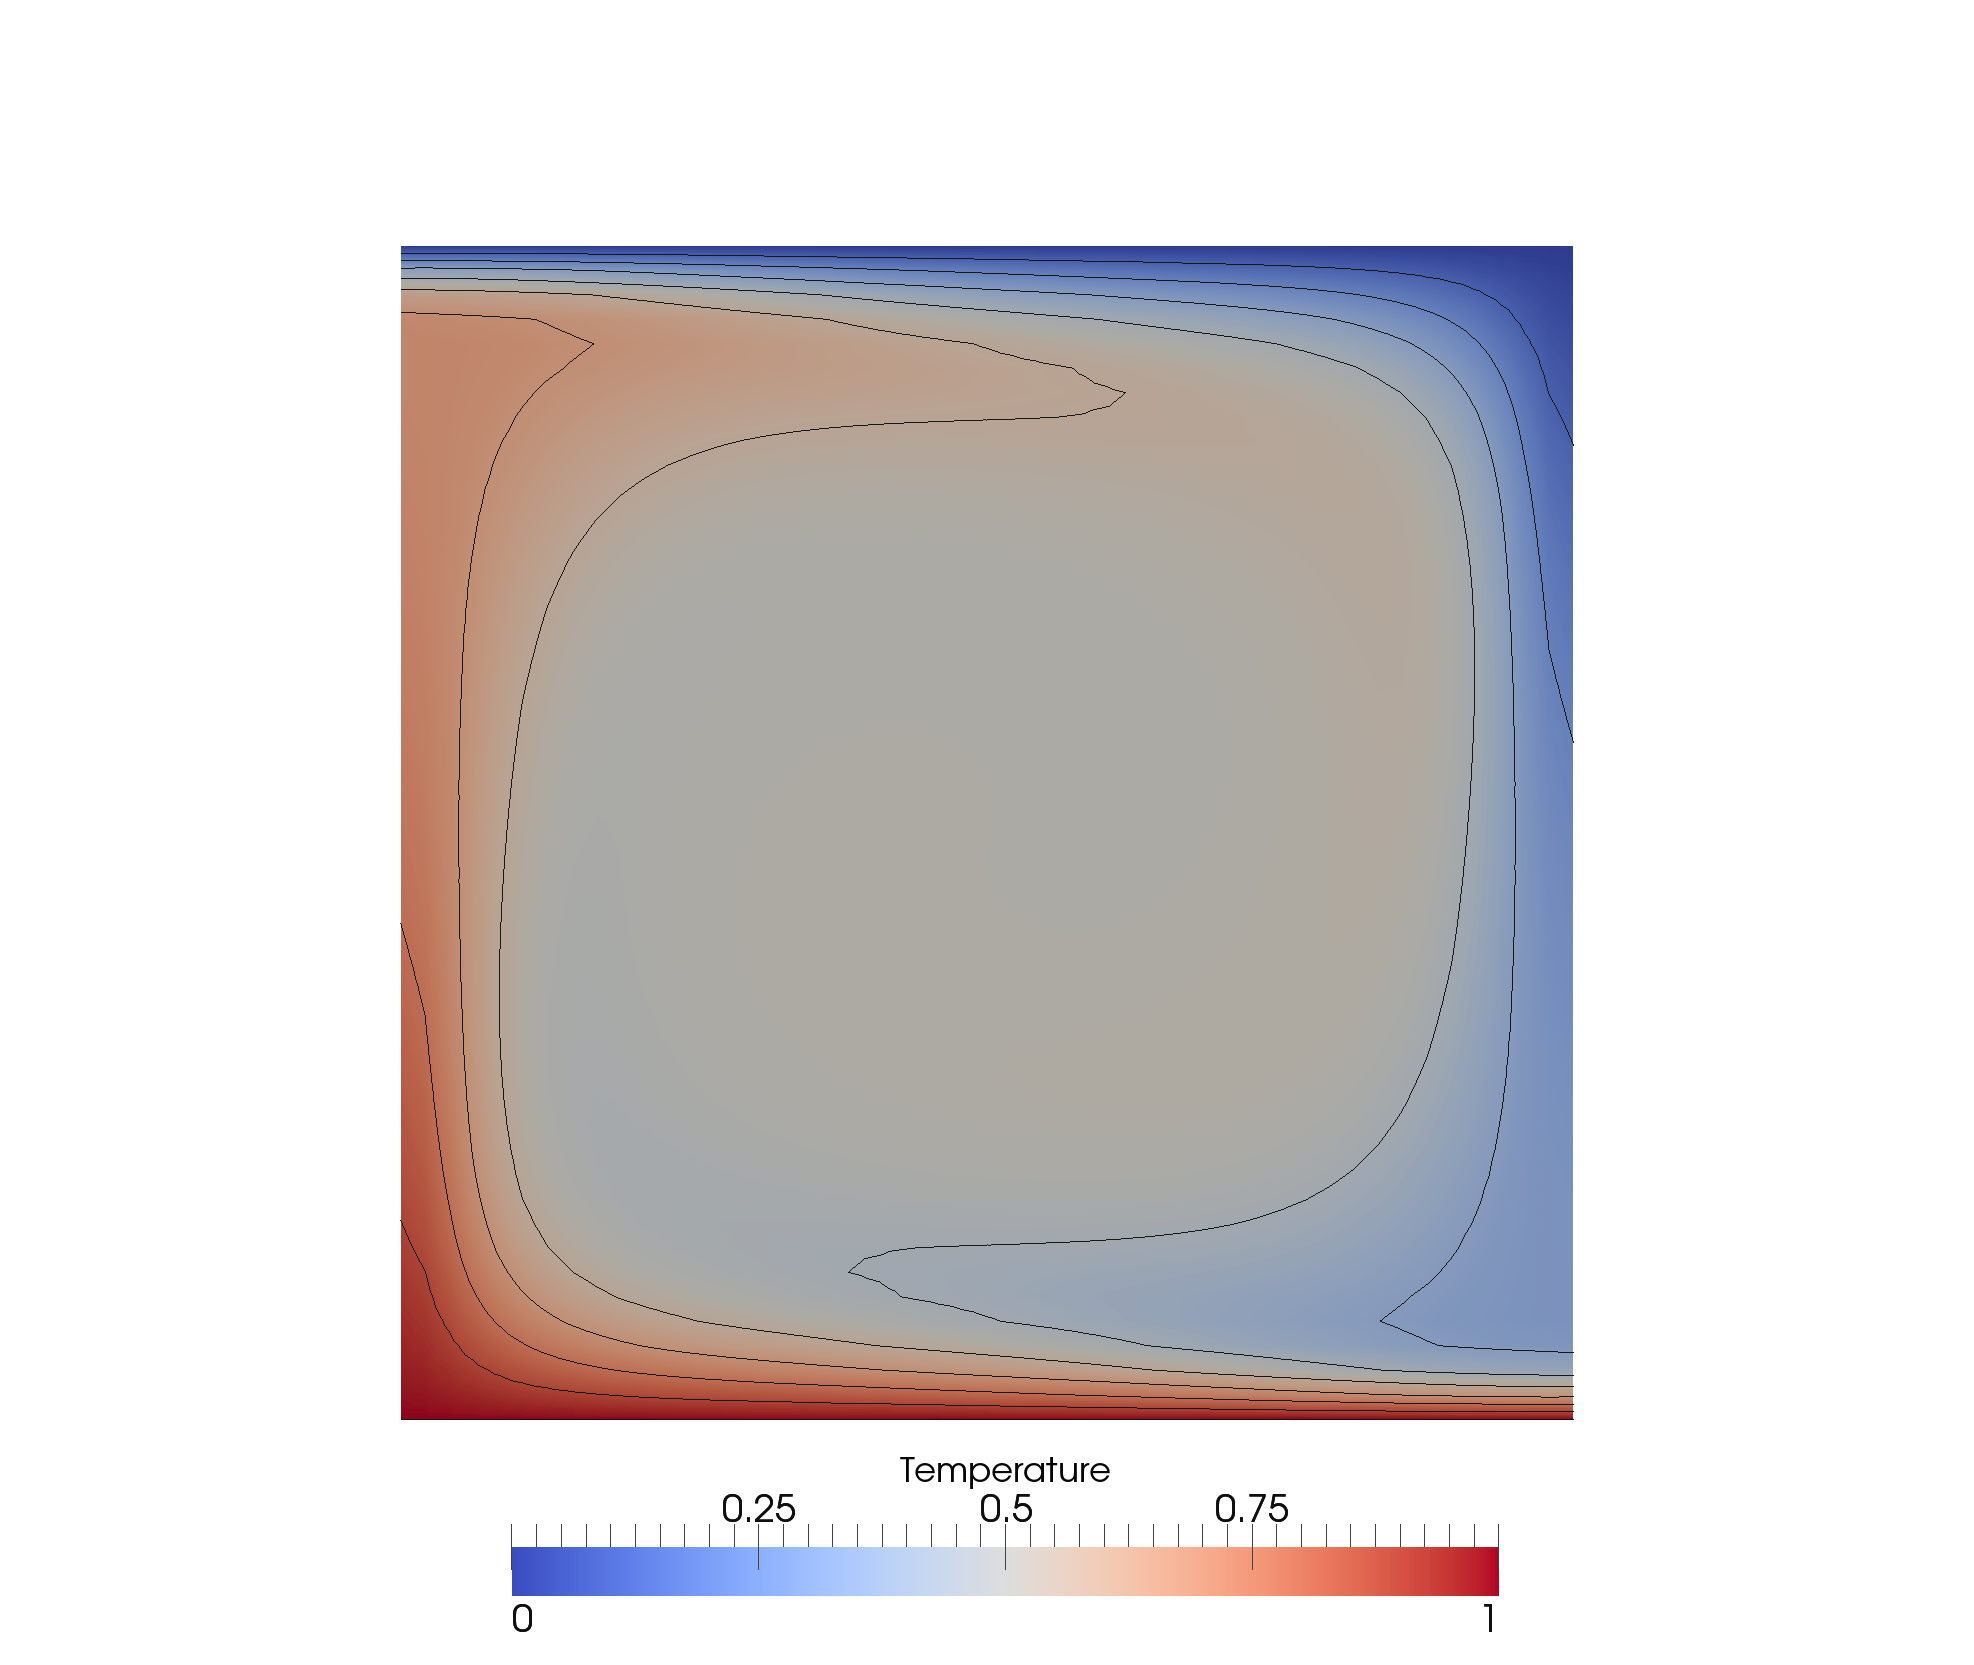
\includegraphics[width=0.5\textwidth]{./stokes_square_convection/Temperature_planform.png}
  \caption{Steady–state temperature field from an isoviscous Stokes simulation at $Ra = 1 \times
    10^5$, on a uniform structured mesh of 48 × 48 elements. Contours are spaced at intervals of
    0.1.}
\end{figure}
\end{frame}
%
\begin{frame}
    \frametitle{Stokes square convection}
\begin{figure}
\centering
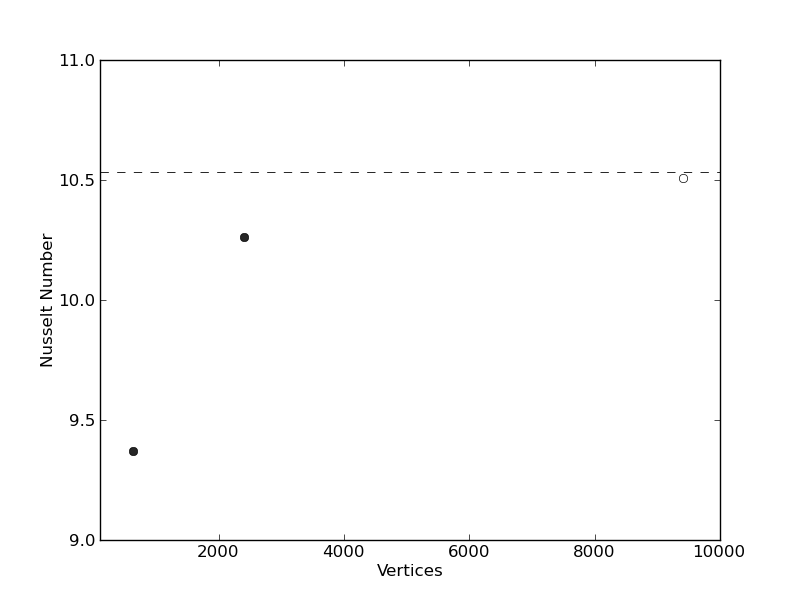
\includegraphics[width=0.5\textwidth]{./stokes_square_convection/Nu_1e5.png}
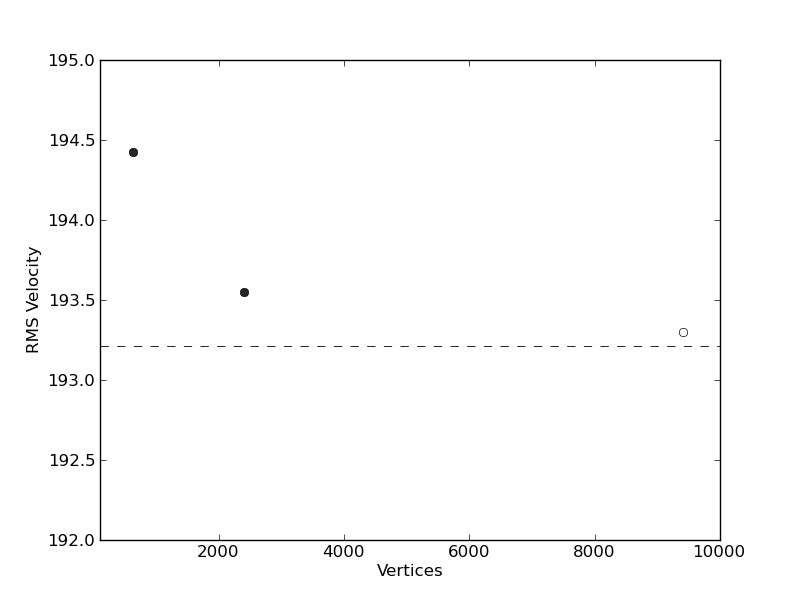
\includegraphics[width=0.5\textwidth]{./stokes_square_convection/RMS_1e5.png}
\caption{Results from 2-D, isoviscous Stokes square convection benchmark cases: (a) Nusselt number
  vs. number of triangle vertices, at $Ra = 1 \times 10^5$, (b) RMS velocity vs. number of triangle
  vertices, at $Ra = 1 \times 10^5$ . Benchmark values are denoted by horizontal dashed lines. Note that the
  highest resolution case is not included in the example.}
\end{figure}
\end{frame}
%
\begin{frame}
    \frametitle{Stokes square convection, exercises}
\begin{itemize}
\item Verify that results do indeed converge towards the benchmark values at higher resolution.
\item Alter the initial condition for temperature to verify that, excluding the location of upwelling
flow at $x = 0$ or $x = 1$, results are insensitive to this initial condition.
\item Change the Rayleigh number to $Ra = 1 \times 10^4$
\end{itemize}
\end{frame}

